  \epigraph{Dlaczego wysoki odsetek pracowników służby drogowej ma rodziny? Bo dużo Hall'ują.}{\textit{Niezwykle suchy żart pewnego studenta}}
  \begin{theorem}[Halla]
      Graf dwudzielny $G = (X,Y,E)$, gdzie $|X|$ = $|Y|$ ma dopasowanie doskonałe wtedy i tylko wtedy, gdy dla dowolnego $A \subset X$ zachodzi: \begin{equation}
          |A| \leq |N(A)|
      \end{equation}
  \end{theorem}

  \begin{proof}
      Ponieważ twierdzenie mówi \textit{wtedy i tylko wtedy}, musimy udowadniać w dwie strony. Zacznijmy od tej prostszej strony, czyli pokażmy że gdy graf dwudzielny w którym $|X| = |Y|$ ma dopasowanie doskonałe to $|A| \leq |N(A)|$. Zasadniczo od razu to widać, bo skoro dopasowanie doskonałe istnieje to wystarczy sobie je wziąć. Każdy wierzchołek z $|X|$ ma wówczas jakąś krawędź do wierzchołka z $|Y|$. Zauważamy, że siłą rzeczy w samym dopasowaniu (czyli jakimś podgrafie oryginalnego grafu dwudzielnego, z którego być może ,,wywalono'' jakieś krawędzie) jest tak, że $|A| = |N(A)|$, z czego w szczególności wynika teza. To chyba widać. 

      W drugą stronę jest ciekawiej, bo po pierwsze musimy sobie wprowadzić instytucję \textit{ścieżki powiększającej}. Nie należy tego mylić ze ścieżką powiększającą z przepływów, bo one mówią o innych rzeczach (ale idea jest ta sama). Generalnie to załóżmy sobie, że mam jakieś dopasowanie $M$ które nie jest doskonałe. Oznacza to, że w $X$ jest jakiś wierzchołek $x_0$ poza dopasowaniem. Jeśli $x_0$ łączy się z jakimś wierzchołkiem $y_0 \in Y$ i $y_0 \in M$. $y$ łączy się z jakimś $x_1 \in M$ (bo są razem w dopasowaniu). Teraz jeśli $x_1$ łączy się z jakimś $y_1 \in Y$ takim, że $y_1 \not \in M$ to ja to dopasowanie mogę przerobić: ,,połączyć'' $x$ z $y$ i $x_1$ z $y_1$, dorzucając dodatkowy wierzchołek do dopasowania. To jest przykład bardzo krótkiej ścieżki powiększającej, ale generalna idea to jest taki ,,zygzak'' którego można przerobić, żeby dopasowanie powiększyło się o jeden wierzchołek. At this point wszyscy już chyba wiedzą, że zamiłowania do formalizmu to ja nie mam. 
      
      \begin{figure}[H]
          \centering
          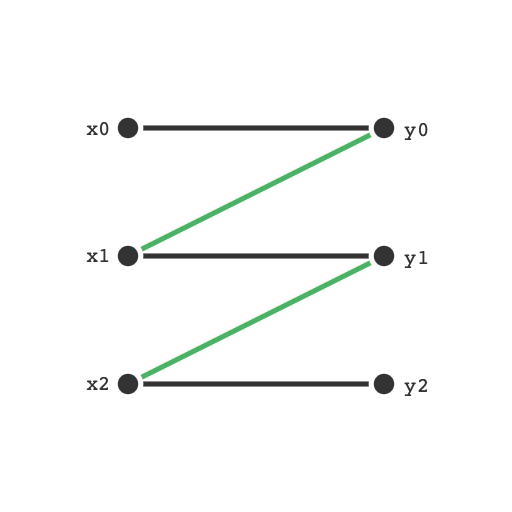
\includegraphics[scale=0.3]{chapters/dyskretna/matchings/images/augmenting_path_before.png}
          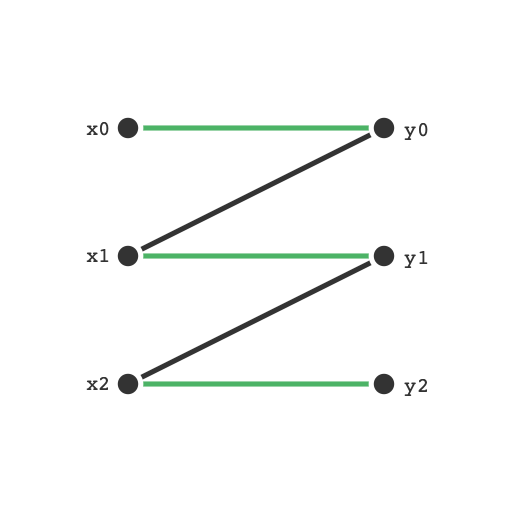
\includegraphics[scale=0.3]{chapters/dyskretna/matchings/images/augmenting_path_after.png}
          \caption{Ścieżka powiększająca przed i po zamianie krawędzi}
      \end{figure}

      No dobra, ale co ma ścieżka powiększająca do twierdzenia Halla? Okazuje się że jest ona bardzo wygodnym narzędziem.

      Załóżmy sobie nie wprost, że mamy jakiś graf dwudzielny $G = (X,Y,E)$, w którym zachodzi warunek Halla ale nie ma dopasowania doskonałego. W takim razie weźmy dopasowanie maksymalne $M$. Istnieje jakiś $x$, który nie należy do tego dopasowania (bo nie jest doskonałe). Z warunku Halla ($|A| \leq |N(A)|$ dla dowolnego $A \subset X$) mam, że $x$ musi mieć jakiegoś sąsiada w $Y$. Zbiór wszystkich wierzchołków, z którymi połączony jest $x$ (być może jest ich więcej, być może tylko jeden) oznaczam jako $B_0$. Każdy wierzchołek z $B_0$ musi należeć do dopasowania $M$ (bo inaczej mógłbym je rozszerzyć, biorąc krawędź między tym wierzchołkiem a $x$). Wszystkie wierzchołki z $X$ które są razem w dopasowaniu z wierzchołkami z $B_0$ oznaczam jako $A_1$. Oczywiście $|A_1| = |B_0|$. Zauważmy, że $|A_1 \cup \{x\}| \geq |B_0|$, a zatem musi istnieć jakiś zbiór wierzchołków $B_1$ który ma krawędzie do wierzchołków zbioru $A_1$. Ponownie, wszystkie krawędzie z $B_1$ muszą być w dopasowaniu, bo inaczej mielibyśmy ścieżkę powiększającą (aha!) od $x$ do jakiegoś wierzchołka z $B_1$. W takim razie mamy jakiś zbiór $A_2$ wierzchołków które są w dopasowaniu z wierzchołkami z $B_1$, ponownie $|A_2| = |B_1|$. $|A_2| + |A_1| + 1 \geq |B_0| + |B_1|$, skąd wierzchołki z $A_2$ łączą się jeszcze z jakimiś innymi wierzchołkami z $Y$, ich zbiór nazwiemy $B_2$. I ponownie, wierzchołki z $B_2$ muszą być w dopasowaniu, bo inaczej mielibyśmy ścieżkę powiększającą. Korzystamy teraz z faktu który zawsze zakładamy, tj. faktu że grafy są skończone.
      
      \epigraph{I tak dalej, aż do wyczerpania zasobów}{\textit{Stefan ,,Siara'' Siarzewski do senatora Ferdynanda Lipskiego, ,,Kilerów-ów 2-óch''}}

      Nietrudno bowiem zauważyć, że w końcu wierzchołki się skończą i albo dostaniemy sprzeczność z założeniem że warunek Halla zachodzi, albo wyjdzie nam ścieżka powiększająca (a dopasowanie miało być maksymalne). Tym samym kończymy dowód. 
  \end{proof}